\documentclass{abnt}
\PassOptionsToPackage{countmax}{subfloat}
\PassOptionsToPackage{hyphens}{url}
\usepackage[brazilian]{babel}
\usepackage{hyperref}
\usepackage[utf8]{inputenc}
\usepackage[T1]{fontenc}
\usepackage[alf]{abntex2cite}
\usepackage{graphicx}
\usepackage{color}
\usepackage{paralist}
\usepackage{subfloat}
\usepackage{subfig}
\usepackage{multirow}
\usepackage{booktabs}
\usepackage{float}
\usepackage{setspace}
\usepackage{tabularx}
\usepackage{array}
\usepackage{longtable}
\usepackage{caption}
\onehalfspacing
\graphicspath{{imagens/}}
% --- Espaçamento ---
\usepackage{setspace}
\onehalfspacing % Espaçamento 1,5

% --- Tabelas ---
\usepackage{booktabs}
\usepackage{tabularx}
\usepackage{array}
\usepackage{longtable}
\usepackage{caption}
% --- Fonte da nota da tabela ---
% --- Correção para habilitar o comando \fonte na classe abnt antiga ---
\newcommand{\fonte}[1]{%
  \par\vspace{2pt}%
  \centering{\small #1}\par
}

\instituicao{UNEB - Universidade do Estado da Bahia 
             \par Departamento de Ciências Exatas e da Terra}
\titulo{Cognitivo: Pensamento Computacional e gamificação no aprendizado de matemática para o Exame Nacional do Ensino Médio (ENEM)}
\autor{Guilherme Dos Santos Modesto Teixeira}
\orientador{Monica de Souza Massa}
\comentario{\textbf{Áreas da Computação:}
           \\  Informática na Educação
           \\ Engenharia de Software
           \\ Desenvolvimento Web}
\local{Salvador-BA}
\date{2 de junho de 2026}
\hyphenation{in-sight}

\begin{document}
\capa
\folhaderosto

\begin{folhadeaprovacao}
\begin{center}
    \large
    \textbf{Folha de Aprovação}
\end{center}

Anteprojeto sob o título provisório Cognitivo: Pensamento Computacional e gamificação no aprendizado de matemática para o Exame Nacional do Ensino Médio (ENEM) apresentado como exigência parcial para avaliação na disciplina Trabalho de Conclusão de Curso I do bacharelado em Sistemas de Informação da Universidade do Estado da Bahia entregue por Guilherme Dos Santos Modesto Teixeira a Marco Antônio Costa Simões, professor da disciplina, em 2 de Junho de 2026, em Salvador, Bahia. 
\setlength{\ABNTsignthickness}{0.4pt}
\setlength{\ABNTsignskip}{2cm}
\hspace*{1cm}
 \assinatura{Guilherme Dos Santos Modesto Teixeira\\Orientando}
\hspace*{1cm}
 \assinatura{Monica de Souza Massa}
\end{folhadeaprovacao}

%\begin{resumo}

%\end{resumo}

\sumario

\chapter{Introdução}
O resultado mais recente do Exame Nacional do Ensino Médio (ENEM) de 2024 demonstra que embora a média geral aumentou de 543 para 546 pontos, a área de Matemática e suas Tecnologias apresentou redução de 535 para 529 pontos \cite{inep2025enem}, sugerindo que a disciplina de matemática apresenta maior dificuldade pelos alunos.

A matriz de referência do ENEM exige que, particularmente na área de Matemática, o estudante deve selecionar, organizar, relacionar, interpretar dados e informações, representados de diferentes formas, para tomar decisões e enfrentar situações problema.\cite{matriz_enem}. 

O ENEM valoriza competências relacionadas à construção de estratégias de resolução de situações-problema. O baixo desempenho em Matemática evidencia dificuldades relacionadas ao raciocínio lógico e à resolução de problemas.

Em uma sociedade que está cada vez mais marcada pelo impacto das tecnologias digitais, é fundamental desenvolver habilidades analíticas que permitam entender, conceber e resolver problemas complexos do mundo real. A cientista da computação Jeannette M. Wing, em seu artigo \textit{Computational Thinking}, publicado em 2006, evidencia a importância do Pensamento Computacional (PC). Essas habilidades convergem com as competências necessárias para o ENEM.

É descrito por \cite{wing2006}, como habilidades que envolvem resolver problemas, projetar sistemas e entender o comportamento humano, utilizando os conceitos fundamentais da ciência da computação. O PC inclui uma gama de ferramentas mentais que refletem a amplitude do campo da ciência da computação.

O processo de abstração consiste em filtrar os aspects importantes. A decomposição,em conjunto, é dividir uma tarefa grande e separar por interesse, facilitando o gerenciamento. Isso permite a criação de soluções de forma algorítmica. Também é descrito por \cite{wing2006} o papel do reconhecimento de padrões para investigar e processar vastas quantidades de dados em busca de similaridades.

Segundo \cite{wing2006} o PC é uma habilidade inerente a todos, não apenas para cientistas da computação. É tão indispensável quanto a leitura, a escrita e a aritmética. É pensar como os humanos resolvem problemas, de forma complementar e integrada ao raciocínio matemático e de engenharia. A autora também argumenta que, quando os conceitos computacionais estiverem integrados no dia a dia, deixarão de ser vistos como uma filosofia explícita.

\begin{citacao}
Não são apenas os artefatos de software e hardware que produzimos que estarão fisicamente presentes em todos os lugares e impactará nossas vidas o tempo todo, serão os conceitos computacionais que usamos para abordar e resolver problemas, gerenciar nossas vidas diárias e nos comunicar e interagir com outras pessoas; e para todos, em todos os lugares. O pensamento computacional será uma realidade quando for tão integral aos esforços humanos que desapareça como uma filosofia explícita \cite[tradução nossa]{wing2006}.
\end{citacao}

No âmbito nacional, a Base Nacional Comum Curricular (BNCC) prioriza a incorporação do PC nas aulas de matemática como uma competência essencial para a modelagem e resolução de problemas \cite{brasil2017}. Dentre elas, destacam-se a decomposição de desafios complexos em partes menores e gerenciáveis, o reconhecimento de padrões, além das práticas de generalização e reúso, permitindo adaptar ou aproveitar uma lógica para resolver novos problemas de forma genérica.

\begin{citacao}
    Decomposição é uma das principais técnicas de resolução de problemas, na qual um problema é dividido em subproblemas, os quais são resolvidos independentemente, e cujas soluções são combinadas para construir a solução do problema original. [...] Em conjunto, deve-se desenvolver o reconhecimento e a identificação de padrões, construindo conjuntos de objetos com base em diferentes critérios [...]. O próximo passo é comparar diferentes casos particulares (instâncias) de um mesmo problema, identificando as semelhanças e diferenças entre eles, e criar um algoritmo para resolver todos [...] de forma genérica. [...] Ao explicar para alguém como realizar uma tarefa (resolver um problema), se está criando um algoritmo. Esses algoritmos podem ser construídos [...] partindo do zero, na qual esses passos também devem ser determinados, além da sequência desses
    \cite{brasil2017}
\end{citacao}
A BNCC também sugere o desenvolvimento do PC nos alunos independente do uso de computadores, com práticas plugadas (jogos digitais, programação em bloco ou textual, simuladores) e experiências desplugadas (usando papel, brincadeiras populares, desenhos e dinâmicas físicas) para exercitar essas habilidades cognitivas \cite{brasil2017}.

Práticas plugadas, especificamente Jogos Sérios, tem um propósito específico relacionado ao treinamento, não apenas para diversão, como descrito por \cite{kiryakova2014gamification}. Eles possuem todos os elementos dos jogos, parecem jogos, mas seu objetivo é alcançar algo que é predeterminado.

O uso de elementos de gamificação com foco em melhorar o engajamento, devem englobar dimensões relacionadas a motivação, objetivos, características da atividade e do usuário, emocional e aspectos cognitivos. Segundo \cite{silpasuwanchai2016developing}, estratégias típicas de jogos no ambiente educacional (pontos, medalhas, desafios e quadros de líderes) tem como objetivo elevar a motivação e, principalmente, o engajamento. Embora o aumento do esforço e da participação tem uma positiva correlação com a melhoria nas notas, a percepção de diversão pelo aluno (engajamento emocional) não se traduz automaticamente em resultados acadêmicos mais altos. Dessa forma, para que a gamificação cumpra seu papel, não deve-se focar apenas em entreter, mas sim estimular um investimento psicológico profundo que conduza à verdadeira aquisição e transferência de habilidades para outros contextos.

O uso de mecânicas de gamificação citadas podem elevar a motivação e engajamento dos estudantes, favorecendo o processo de aprendizagem e, consequentemente, a melhoria do desempenho em avaliações como ENEM. É necessário usar a gamificação para focar na aquisição do conhecimento, desenvolvendo as habilidades do PC com foco em estruturar raciocínio para resolução de problemas. Como o ENEM prioriza estratégias de resolução de problema. Essa abordagem poder tornar o ensino da matemática mais lúdico e contextualizado.

Na revisão sistemática da literatura, ficou evidente que parte das práticas gamificadas no contexto da Matemática falham ao não desenvolver o raciocínio com PC, limitando-se ao aspecto lúdico. Alinhados a essa realidade, os conceitos citados fundamentam a elaboração deste anteprojeto, cuja proposta parte do baixo desempenho dos estudantes em matemática no ENEM para criação do sistema gamificado, fundamentado nos pilares do PC, que pode engajar estudantes do 3º ano do Ensino Médio. Esse cenário evidencia a necessidade em desenvolver competências associadas ao PC, que alinham-se às diretrizes da BNCC.

\chapter{Objetivos}
O objetivo geral consiste em desenvolver e avaliar um sistema gamificado, fundamentado nos pilares do Pensamento Computacional, que pode engajar estudantes do 3º ano do Ensino Médio.

Para alcançar o objetivo geral é necessário:  
\begin{itemize}
    \item Mapear as principais competências matemáticas das questões do ENEM e como o Pensamento Computacional é desenvolvido.
    \item Conceber e testar sistema gamificado que operacionalize a abstração, decomposição, reconhecimento de padrões e algoritmos no contexto das questões de matemática do ENEM.
    \item Validar do artefato educacional com professores de matemática do curso de Sistemas De Informação.
    \item Avaliar a experiência dos estudantes com Modelo de Amostragem de Experiência (ESM) e Escala de Engajamento do Usuário (UES).
\end{itemize}

\chapter{Justificativas e Contribuições}
Diante do cenário exposto na introdução deste documento, evidencia-se a necessidade de estratégias pedagógicas que fortaleçam o ensino de Matemática, especialmente no que se refere ao desempenho dos estudantes em Matemática no ENEM. Nesse contexto, o Pensamento Computacional (PC), alinhado às diretrizes da Base Nacional Comum Curricular (BNCC), destaca-se como uma abordagem relevante para o desenvolvimento de habilidades para resolução de problemas dos alunos.

Neste sentido, a proposta busca integrar esses referenciais em um ambiente de aprendizagem real. Assim, espera-se contribuir para a melhoria do processo de aprendizagem, investigando como a articulação entre PC e gamificação pode impactar positivamente o desempenho dos estudantes no ENEM.

\chapter{Metodologia}
Uma pesquisa qualitativa é descrita por \cite{yin2016pesquisa} como uma investigação com capacidade de entender, traduzir e valorizar as visões dos sujeitos envolvidos diretamente no fenômeno estudado. É capturar as perspectiva dos participantes.

Nesse sentido, a pesquisa caracteriza-se pelo caráter qualitativo, pois foca nos significados e nas percepções de professores e alunos ao longo da intervenção pedagógica. 

É fundamental abranger dimensões sociais, institucionais e ambientais, nas quais a vida humana se desenrola. Esses fatores exercem profunda influência sobre os comportamentos e eventos investigados.\cite{yin2016pesquisa}. 

A metodologia Design-Based Research (DBR), amplamente utilizada na criação de práticas educacionais, serve como base para o desenvolvimento deste estudo. Essa metodologia oferece uma estrutura que permite a elaboração de artefatos pedagógicos dirigidos à intervenção e solução de problemas no âmbito educacional. Tendo em vista que o propósito deste anteprojeto de pesquisa é estruturar o desenvolvimento de um sistema para contextos educacionais, a DBR se estabelece como o fundamento deste estudo.

A DBR é definido por \cite{plomp2018pesquisa} como uma abordagem colaborativa e iterativa ou uma família de abordagens de pesquisa, não apenas como metodologia estrita. Fundamenta-se em aspectos como projetar e produzir soluções no contexto educacional e aprofundar o conhecimento científico sobre essas intervenções, criando alicerce teórico ou princípios de design e gerar futuras aplicações.

De acordo com \cite{plomp2018pesquisa}, essas intervenções dirigidas à resolução de problemas práticos não se limitam a mudanças curriculares, abrangendo explicitamente a formulação de artefatos pedagógicos, materiais, produtos e sistemas voltados para a educação. É pragmática, intervencionista e colaborativa, pois pesquisadores e profissionais da educação podem trabalhar juntos.

\begin{citacao}
    intervencionista: a pesquisa objetiva a elaboração de uma intervenção para uma situação da vida real [...] envolvimento dos praticantes: a pesquisa envolve a participação ativa ou a colaboração com os praticantes em vários estágios e atividades da pesquisa — isto aumenta a chance de que a intervenção se torne, de fato, relevante e prática para o contexto educacional [...] O design é caracterizado por sua ênfase nas soluções, guiadas por propósitos mais amplos e metas ideais. Além disso, o design desenvolve e projeta propostas que são testadas em experimentos pragmáticos e fundamentadas na ciência educacional [...] \cite{obrien2018practical}
\end{citacao}

A DBR define fases que consistem em identificar o problema, propor o desenvolvimento de soluções, ciclos de aplicação e refinamento iterativos. Por fim, reflexões e melhorias.

O fluxo a seguir descreve as etapas e as estratégias empregadas para o desenvolvimento da intervenção.

\begin{figure}[H]
    \centering
    \caption{Fluxo geral do DBR}
    \label{fig:fluxo-geral-dbr}
    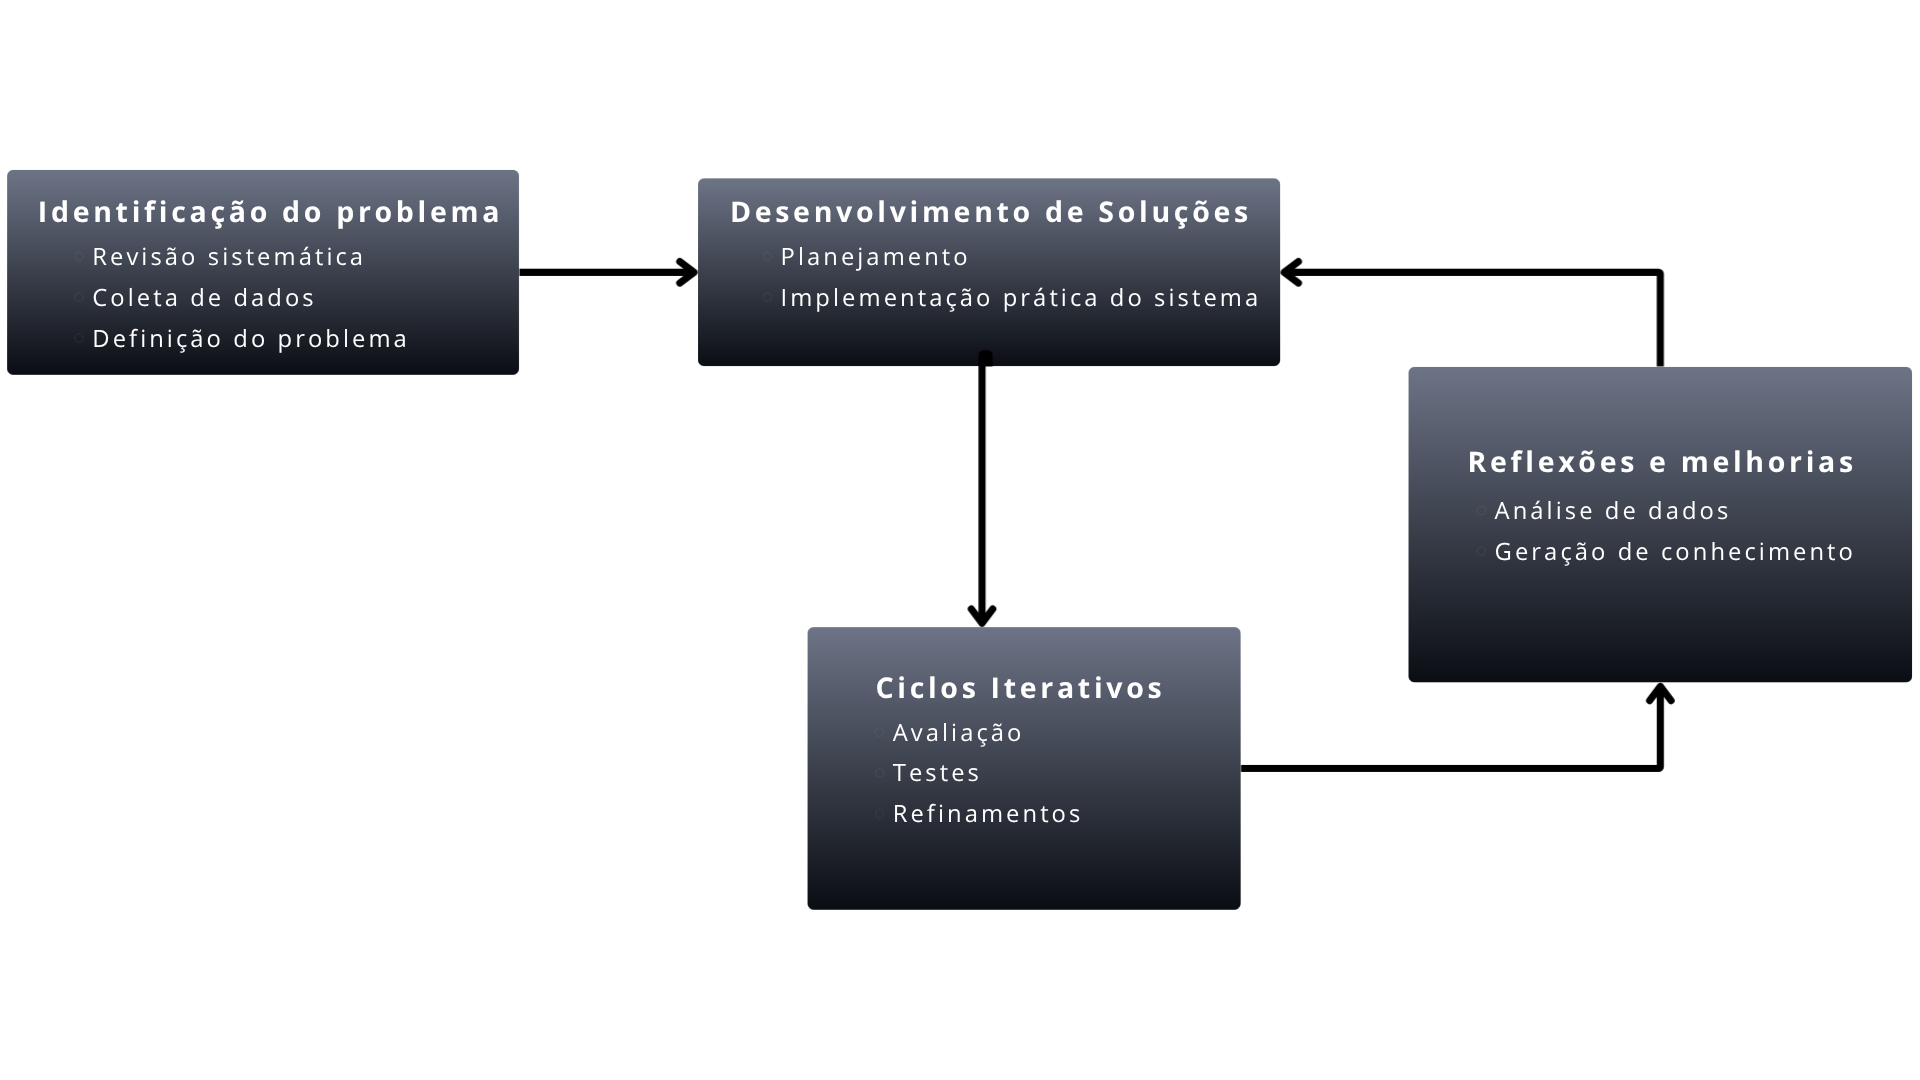
\includegraphics[width=\textwidth]{Fluxo_Geral_DBR.png}
    \fonte{Elaborado pelo autor (2026).}
\end{figure}

A operacionalização da pesquisa encontra-se na tabela abaixo, que correlaciona as fases conceituais da (DBR) com os entregáveis do desenvolvimento do projeto.

\renewcommand{\tablename}{Quadro}
\renewcommand{\arraystretch}{1.5} 
\begin{longtable}{
    | >{\bfseries\raggedright\arraybackslash}p{4.0cm} 
    | >{\raggedright\arraybackslash}p{10.5cm} |}
    \caption{Etapas do DBR e seus respectivos desenvolvimentos} \label{quadro:dbr} \\
    \hline
    \normalfont\bfseries Etapas do DBR &
    \normalfont\bfseries Etapas de Desenvolvimento \\
    \hline    \endhead
 
    Identificação do problema &
    Revisão Sistemática de Literatura. Mapear as principais
    competências matemáticas das questões do ENEM e como o
    Pensamento Computacional é desenvolvido. \\
    \hline
 
    Desenvolvimento de soluções &
    Definição da arquitetura e das mecânicas de gamificação
    da plataforma. Desenvolvimento da
    primeira versão funcional da plataforma. \\
    \hline
 
    Ciclos iterativos &
    Ciclo 1:Avaliação por professores de Matemática do curso de
    Sistemas de Informação.
    Ciclo 2: Avaliação por alunos da UPT.\\
    \hline
 
    Reflexões e melhorias &
    Ciclo 1: Refinamento do sistema a partir do feedback dos professores.
    Ciclo 2: Uso de sistema pelos alunos e aplicação dos formulários ESM e UES. Analisar os dados dos
    formulários e geração de conhecimento. \\
    \hline
\end{longtable}

\begin{center}
    \vspace{-0.5cm}
    {\small Fonte: Elaborado pelo autor (2026).}
\end{center}

\section{Identificação do problema}
\sloppy

A etapa inicial da metodologia DBR é a investigação preliminar, descrito por \cite{obrien2018practical}, como parte essencial para obter um insight profundo sobre o problema educacional, compreendendo a situação-problema e as possibilidades de inovação.
Em relação ao referencial teórico, a revisão sistemática de literatura implementada formaliza esse processo, explorando bases de conhecimento, avaliando intervenções ou projetos sobre a temática do Pensamento Computacional e gamificação para o contexto da aprendizagem em matemática. O contexto do problema consiste em argumentar sobre o baixo desempenho em matemática no ENEM e a falta de práticas voltadas para o tema.

\section{Ciclos Iterativos de Avaliação}
Os ciclos iterativos e de avaliação, de acordo com \cite{obrien2018practical} são testes e refinamentos das soluções. Esse processo, na prática, é repetido até que alcance um equilíbrio entre o que foi idealizado e a produção. É feito uma avaliação formativa a cada ciclo, pois é o motor que impulsiona o avanço.

A etapa de ciclos iterativos é dividida em duas etapas: Ciclos de validação por especialistas e aplicação com alunos.
\subsection{Ciclo de validação por especialistas}

Grupo focal é descrito por \cite{gil2021pesquisa} como um tipo especial de grupo em termos de finalidade, tamanho, composição e procedimentos. Um grupo focal não busca consenso, mas encoraja a expressão de respostas que possibilitam uma melhor compreensão das atitudes, comportamentos, opiniões e percepções dos participantes. Caracteriza-se pelo uso explícito da interação para gerar dados.

Segundo \cite{gil2021pesquisa}, o planejamento do grupo focal é uma das estratégias mais estruturadas entre as variadas abordagens empregadas na coleta de dados em pesquisas qualitativas, exigindo que o pesquisador faça uma série de decisões rigorosas. Os participantes devem estar em consonância com os objetivos da pesquisa.

O grupo focal será composto pelos especialistas em matemática do curso de Sistemas de Informação, uma vez que a experiência dos professores os torna aptos para avaliar a viabilidade pedagógica do sistema.

Validação com professores de matemática do curso de Sistemas De Informação, focando no \textit{feedback}. Segundo \cite{plomp2018pesquisa} descreve que o protótipo deve ser submetido a revisões e refinamentos a partir da avaliação dos especialistas, para que as intervenções educacionais ultrapassem a idealização teórica, e que sua aplicabilidade e sua capacidade de sobreviver e funcionar de maneira efetiva frente às condições, desafios e restrições reais do contexto educacional e do "chão da escola".

A avaliação do sistema por parte dos professores será conduzida com foco na validação dos conteúdos matemáticos, verificando se os enunciados, dados e gabaritos mantêm a acurácia e o rigor conceitual exigidos. Como o sistema trata e processa essas demandas cognitivas e se as mecânicas de gamificação foram projetados de modo a induzir e estimular o raciocínio. 

\subsection{Ciclo de validação por alunos}
Os ciclos de validação pelos alunos tem como objetivo aferir se o produto resultou nos impactos e nas consequências de aprendizagem desejados e como a intervenção afeta o raciocínio, compreensão, criatividade, atitude e a motivação dos alunos, como descrito por \cite{plomp2018pesquisa}.

Nessa etapa serão aplicados os formulários de Método de Amostragem de Experiência (ESM) e Escala de Engajamento do Usuário (UES).

\subsubsection{Método de Amostragem de Experiência (ESM)}
O método de amostragem de experiência é utilizado para medir a experiência do usuário ao utilizar um sistema, coletando informações durante o uso. É descrito por \cite{francisco2020esm}, como investigações que necessitam coletar dados de uma experiência que ocorreu com base em um evento específico para entender como os participantes interagem com o sistema.

O uso desse método fundamenta-se na necessidade de garantir a adesão dos participantes, pois os usuários são mais dispostos a responder quando o questionário é curto, simples, fácil de compreender e responder, não exigindo muito esforço mental \cite{francisco2020esm}.

A aplicação do método consiste na criação do formulário de amostragem da experiência do usuário, utilizando a Escala Likert com campos de resposta com radio buttons, checkboxes e campos abertos. 

De acordo com \cite{francisco2020esm}, a criação do formulário deve considerer a possibilidade de resposta em menos de um minuto. A agilidade deve ser garantida por meio de campos de resposta rápida. Quando o objetivo for medir o grau de concordância com uma afirmação, deve-se preferir o uso de escalas menores, como a de 5 pontos, visto que escalas maiores fazem o participante parar para pensar. Por outro lado, os campos abertos devem ser evitados ou minimizados ao máximo, pois podem tornar a entrada de dados cansativa.

Por fim, \cite{francisco2020esm} destaca que o sucesso da coleta depende de uma configuração técnica voltada para o imediatismo da emoção sentida no jogo. Estabelecer esse limite máximo de tempo para o preenchimento é essencial a fim de garantir que o dado coletado reflita a experiência do momento e não após a sua ocorrência.

\subsubsection{Escala de Engajamento do Usuário (UES)}
A escala de engajamento do usuário é o critério para medição do engajamento e é divido em dimensões, descrito por \cite{obrien2018practical}, que estabelece o instrumento de medição composto por doze questões e quatro dimensões estruturais: Atenção Focada, Usabilidade Percebida, Apelo Estético e Recompensa.

Segundo \cite{obrien2018practical} a atenção focada reflete estado em que o indivíduo se sente pela experiência interativa. A usabilidade percebida envolve a relação entre nível de esforço, sendo a percepção do nível de controle e a quantidade de esforço que o usuário precisa investir para realizar sua tarefa. O apelo estético avalia o nível de atratividade e o apelo visual proporcionados pela interface. 

A dimensão referente a recompensa caracteriza-se pelos aspectos do resultado experiencial, consolidando sucesso geral da interação e a disposição do usuário em recomendar o sistema (durabilidade), o interesse e a curiosidade despertados durante o uso (novidade), além da sensação lúdica de ter se divertido e sido atraído pela experiência (envolvimento sentido) \cite{obrien2018practical}.

No formulário é usado a Escala de Likert como instrumento de medição do nível de concordância das respostas. Nessa avaliação, o participante deve refletir sobre a sua experiência com o sistema e selecionar um valor que varia de 1 (Discordo Totalmente) até 5 (Concordo Totalmente) para cada item.

Conforme \cite{obrien2018practical}, durante a aplicação do instrumento de avaliação, o participante deve refletir acerca de sua experiência interativa com o sistema e indicar seu nível de concordância para cada afirmação.

Em relação ao processo de aplicação do formulário, \cite{obrien2018practical} destaca que a aplicação do formulário deve ser apresentado de maneira misturada e aleatória, sendo estritamente necessário que os identificadores originais das dimensões fiquem ocultos ao respondente. 
\newpage
No momento da apuração dos resultados para o cálculo de fato, os autores ressaltam que o passo primário e obrigatório é realizar a inversão das notas (método de reverse code) das questões negativas pertencentes à Usabilidade Percebida.

\begin{citacao}
Inverta a codificação dos seguintes itens: PU-S1, PU-S2, PU-S3. [...] As pontuações para cada uma das quatro subescalas podem ser calculadas somando os valores das respostas para os três itens contidos em cada subescala e dividindo por três. [...] Uma pontuação geral de engajamento pode ser calculada somando todos os itens juntos e dividindo por doze \cite{obrien2018practical}
\end{citacao}

Por fim, a pontuação específica de cada subescala é extraída a partir da média aritmética simples, enquanto o escore do engajamento geral do indivíduo é obtido pela soma de todas as doze respostas finais da avaliação.

\section{Desenvolvimento de Soluções}
Definido o problema, a implementação da revisão da literatura e o estudo da metodologia DBR. A solução parte da elaboração do diagrama de caso de uso, da arquitetura e da criação do design da aplicação.

\subsection{Diagrama de Caso de Uso}
O Diagrama de caso uso retrata o comportamento funcional da plataforma educacional gamificada sob a perspectiva das interações dos usuários com o sistema, delimitando claramente a fronteira da aplicação e as regras lógicas que regem o fluxo de aprendizagem. É descrito por \cite{sommerville2011} como uma técnica de descoberta de requisitos, descrevendo o que o usuário espera do sistema, sendo uma ferramenta altamente eficaz para trabalhar com os \textit{stakeholders} que irão interagir diretamente com o \textit{software}.

O ator Estudante relaciona-se com os casos de uso de Autenticar Usuário, responsável por gerenciar o controle de acesso, e Iniciar Sessão de Estudo, que estabelece o início de uma nova trilha de exercícios.

Visualizar Progresso, funcionalidade que renderiza estatísticas de uso na plataforma: nível, posição na liga global, \textit{badges}, sequência de dias ativos e níveis de engajamento por assuntos.
\newpage
O núcleo da plataforma é centralizado no caso de uso Resolver Questão. O sistema guia o aluno pelas fases Abstrair Dados, Decompor Enunciado, Reconhecer Padrão e Criar Algoritmo. O estudante pode treinar cada pilar separado, por isso a relação \textit{extend}. 

O Estudante pode acionar o caso de uso Solicitar Dica quando encontrar dificuldades em cada nível. Com o erro, o sistema calcula de forma proporcional a penalidade via caso de uso Aplicar Penalidade XP.

\begin{figure}[H]
    \centering
    \caption{Diagrama de Caso de Uso}
    \label{fig:diagrama-caso-uso}
    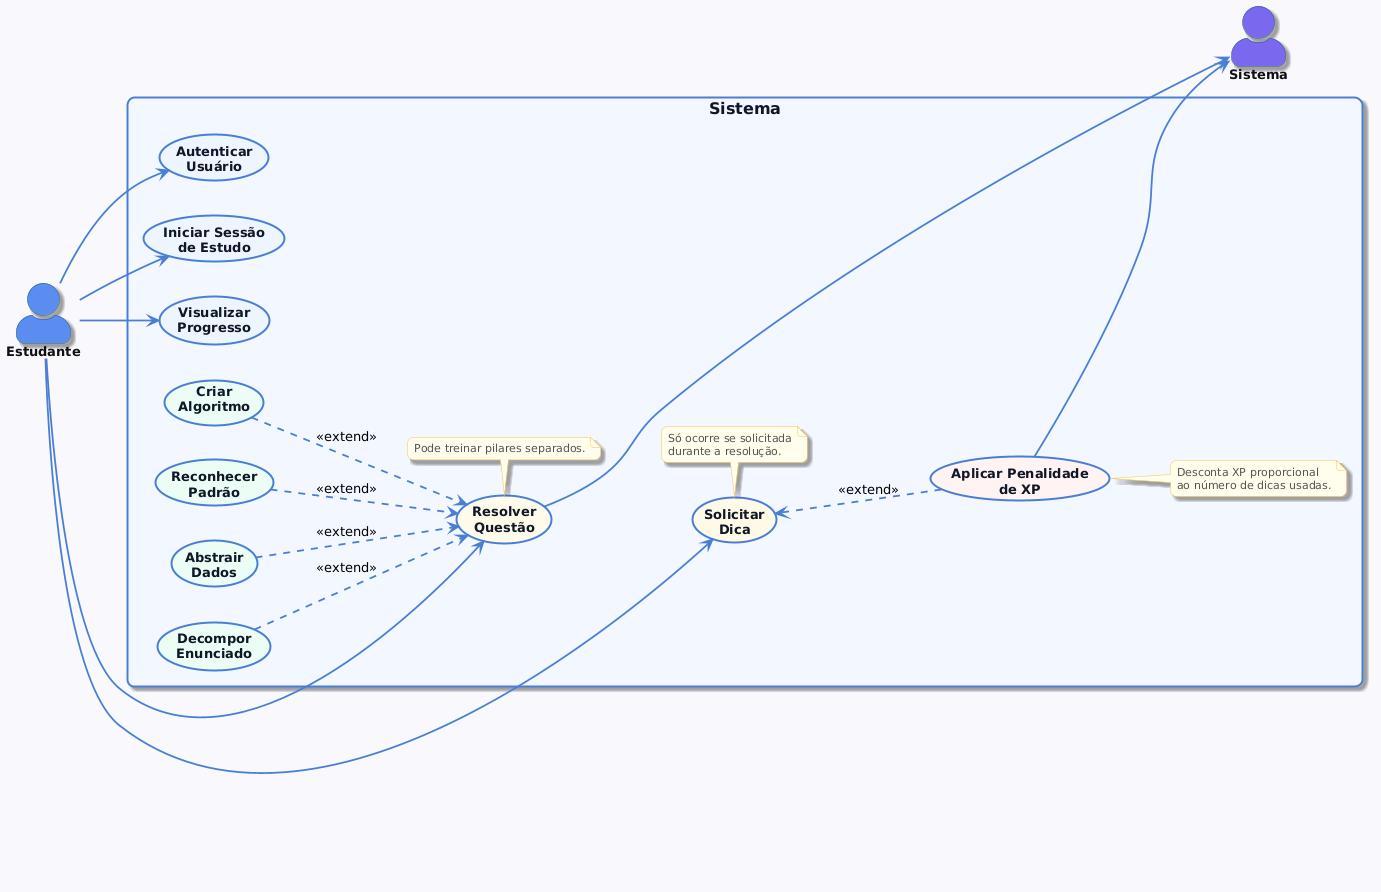
\includegraphics[width=\textwidth]{Diagrma_de_Caso_De_Uso.png}
    \fonte{Elaborado pelo autor (2026).}
\end{figure}

\subsection{Arquitetura do Sistema}
Segundo \cite{brown_c4_model_book}, a arquitetura de um Sistema de Software é uma estrutura composta por contêineres. Esses Contêineres consistem em diversas aplicações e armazenamentos de dados que, juntos, integram o sistema, englobando esquemas de banco de dados, aplicativos móveis, aplicações de console e aplicações web executadas tanto no lado do servidor quanto no cliente. 

\begin{figure}[H]
    \centering
    \caption{Diagrama de Arquitetura}
    \label{fig:diagrama-arquitetura}
    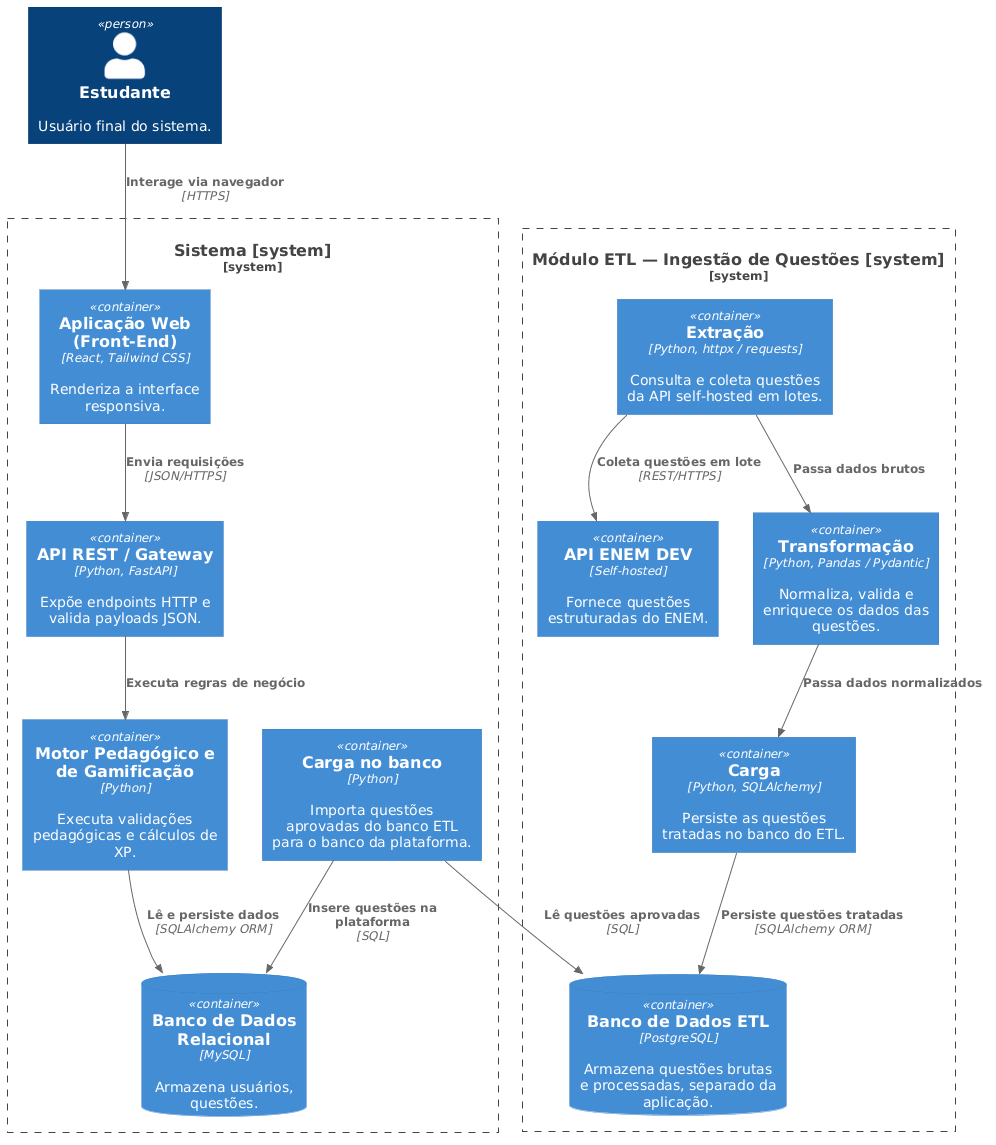
\includegraphics[width=0.95\textwidth]{diagrama_arquitetura.png}
    \fonte{Elaborado pelo autor (2026).}
\end{figure}
O estudante atua como o ator principal, interagindo via protocolo \textit{HTTPS} por meio de seu navegador com a aplicação web construída em \textit{React} e \textit{Tailwind CSS}, renderizando a interface responsiva da plataforma. As requisições em formato \textit{JSON/HTTPS} para a \textit{API REST / Gateway} baseada em \textit{Python} e \textit{FastAPI}. Uma vez validados, os dados fluem para o Motor Pedagógico e de Gamificação, implementado em \textit{Python} que centraliza as regras de negócio do sistema. Para garantir a persistência e a recuperação dos dados de progresso e usuários, este motor se comunica com o Banco de Dados Relacional (\textit{MySQL}) por meio do objeto-relacional com o \textit{SQLAlchemy ORM}.

O módulo \textit{Extract, Transform, Load} (ETL) de Ingestão de Questões, cujo fluxo inicia no container de Extração. Utilizando rotinas em \textit{Python} com as bibliotecas \textit{httpx} e \textit{requests}. As consultas e coletas em lote a uma instância \textit{self-hosted} da \href{https://enem.dev/}{API ENEM DEV} . Os dados brutos são encaminhados para o container de Transformação, no qual scripts em \textit{Python} usando bibliotecas como \textit{Pandas} e \textit{Pydantic} realizam a normalização, validação e o enriquecimento das informações. Em seguida, os dados normalizados alimentam o container de Carga para persistir os dados em banco \textit{PostgreSQL}.

\subsection{Design}
O design da aplicação é fundamentado em princípios de usabilidade, acessibilidade e engajamento, visando proporcionar uma experiência intuitiva e motivadora para os estudantes. A interface é projetada para ser limpa e organizada, com uma paleta de cores que favorece a leitura e a concentração.

De acordo com \cite{preece2013design}, o design deve ser implementado com uma preocupação central em desenvolver produtos interativos que sejam utilizáveis, sendo fáceis de aprender, eficazes no uso. É proporcionar uma experiência agradável.

A interface da aplicação é desenvolvida com foco na simplicidade e na clareza, utilizando uma estrutura de navegação intuitiva. Os elementos visuais são organizados de maneira a guiar o usuário através das diferentes etapas do processo de resolução de problemas, destacando as mecânicas de gamificação para incentivar o engajamento. Esse processo busca atender as metas de usabilidade. É descrito por \cite{preece2013design}, para ser eficaz, eficiente, segura no uso, boa utlidade, fácil de aprender e fácil de lembrar.

Segundo \cite{preece2013design} eficácia é quanto um sistema é bom no que se propõe. A eficiência refere-se como o sistema auxilia o usuário a realizar suas tarefas com o mínimo de esforço. A segurança no uso é a capacidade do sistema de prevenir erros e minimizar as consequências de erros inevitáveis. A boa utilidade é a capacidade do sistema de fornecer as funcionalidades necessárias para os usuários alcançarem seus objetivos. A facilidade de aprendizado é a rapidez com que os usuários podem aprender a usar o sistema. A facilidade de lembrar é a capacidade do sistema de permitir que os usuários se lembrem de como usá-lo após um período de não uso .

O fluxo de navegabilidade abaixo retrata a sequência de passos feitas pelo usuário no sistema e será validado nos cilcos iterativos descritos anteriormente.
\begin{figure}[H]
    \centering
    \caption{Fluxo de navegabilidade}
    \label{fig:design}
    \includegraphics[width=0.95\textwidth]{Fluxo de navegabilidade Final.png}
    \fonte{Elaborado pelo autor (2026).}
\end{figure}

\newpage
\section{Reflexão e melhorias}
O processo de reflexão e melhorias consiste em fazer uma avaliação para o aperfeiçoamento do sistema ao longo de ciclos iterativos e dos formulários de ESM e UES. 

O primeiro ciclo possibilita diagnóstico detalhado, oferecendo o arcabouço conceitual necessário para que o pesquisador entenda a origem de um problema ou falha de design na plataforma. 

Segundo \cite{obrien2018practical}, na prática do ambiente educacional, essa melhoria contínua materializa-se por meio de microciclos, nos quais os pesquisadores elaboram conjecturas prévias, implementam as atividades instrucionais e realizam reflexões com base nas reações e nos resultados reais observados nos alunos. É necessário também, ao final de um experimento ou do teste de um protótipo completo, conduzir uma análise retrospectiva profunda sobre todo o conjunto de dados coletados.

A reflexão sistemática, descrita por \cite{obrien2018practical}, aliada à documentação explícita de todas as decisões que confere o rigor científico à metodologia e permite gerar conclusões que são convertidas em novo arcabouço teórico e prático, que retroalimentam a solução em questão e promovem o progresso no campo de estudo, gerando referência para trabalhos futuros.

\chapter{Cronograma}
O cronograma deste projeto é apresentado no quadro abaixo.

\begin{table}[ht]
    \centering
    \begin{tabular}{ p{6.6cm} c c c c c c }
        \toprule
                   & Mês 1 & Mês 2 & Mês 3 & Mês 4 & Mês 5 & Mês 6 \\
        \midrule
           Definição do problema 
                   & $\bullet$ & $\bullet$ &  &  &  &  \\
        \midrule
           Revisão sistemática de literatura e definição da metodologia  
                   &  & $\bullet$ & $\bullet$ & $\bullet$ &   &  \\
        \midrule
           Diagramas de caso de uso, arquitetura e design da aplicação
                   &  &  & $\bullet$ & $\bullet$ & $\bullet$   &  \\
        \midrule
           Monografia Parcial
                   &  &  &  &  & $\bullet$ & $\bullet$ \\    
        \midrule
           Front-End da aplicação
                   &  &  &  &  & $\bullet$ & $\bullet$ \\
        \midrule
           ETL
                   &  &  &  &  & $\bullet$ & $\bullet$ \\
        \midrule
           Diagrama ER, banco de dados e back-end
                   &  &  &  & $\bullet$ & $\bullet$ & $\bullet$ \\
        \midrule 
           Mecânicas de gamificação
                   &  &  & $\bullet$ & $\bullet$ & $\bullet$ & $\bullet$ \\
        \midrule 
           Infraestrutura 
                   &  &  &  & $\bullet$ & $\bullet$ & $\bullet$ \\
        \bottomrule   
    \end{tabular}
    \caption{Cronograma de Desenvolvimento - Parte 1}   
    \label{tab:cronograma-1-2}
\end{table}

\begin{table}[hb]
    \centering
    \begin{tabular}{ p{7.5cm} c c c c c }
        \toprule
                   & Mês 7 & Mês 8 & Mês 9 & Mês 10 & Mês 11 \\
        \midrule
            Ciclos iterativos de testes e refinamentos com alunos e professores 
                   & $\bullet$ & $\bullet$ & $\bullet$ &  &  \\
        \midrule
           Análise dos resultados
                   &  &$\bullet$& $\bullet$ & $\bullet$ & \\
        \midrule
           Escrita, revisão e monografia final
                   &  & &  & $\bullet$ & $\bullet$ \\
        \bottomrule   
    \end{tabular}   
    \caption{Cronograma de Desenvolvimento - Parte 2}   
    \label{tab:cronograma-2-2}
\end{table}

\bibliographystyle{abnt-num}
\bibliography{referencias}

\end{document}